\begin{figure}[htbp]
\centering
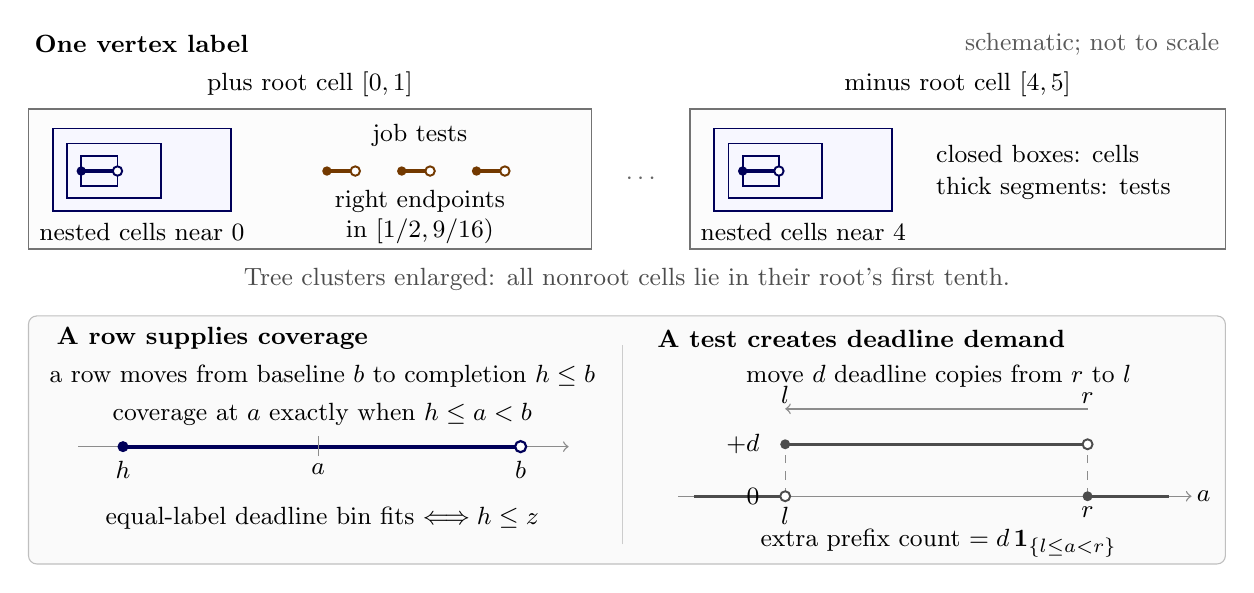
\begin{tikzpicture}[
  x=1cm,y=1cm,
  font=\fontsize{9.5}{11.5}\selectfont,
  every node/.style={inner sep=2pt},
  rootcell/.style={draw=black!55,line width=.6pt,fill=black!1},
  treecell/.style={draw=blue!35!black,line width=.65pt,fill=blue!3},
  test/.style={draw=blue!35!black,line width=1.5pt},
  jobtest/.style={draw=orange!45!black,line width=1.5pt},
  guide/.style={draw=black!45,line width=.5pt},
  heading/.style={font=\fontsize{9.5}{11.5}\selectfont\bfseries}
]
\node[heading,anchor=west] at (.15,6.65) {One vertex label};
\node[anchor=east,text=black!65] at (15.35,6.65)
  {schematic; not to scale};
\node at (3.725,6.14) {plus root cell $[0,1]$};
\node at (11.95,6.14) {minus root cell $[4,5]$};
\draw[rootcell] (.15,4.05) rectangle (7.30,5.83);
\draw[rootcell] (8.55,4.05) rectangle (15.35,5.83);
\node[text=black!60] at (7.925,4.94) {$\cdots$};

\foreach \offset in {0,8.40} {
  \begin{scope}[xshift=\offset cm]
    \draw[treecell] (.46,4.53) rectangle (2.72,5.58);
    \draw[treecell] (.64,4.70) rectangle (1.83,5.39);
    \draw[treecell] (.82,4.85) rectangle (1.28,5.23);
    \draw[test] (.82,5.04) -- (1.28,5.04);
    \fill[blue!35!black] (.82,5.04) circle (1.7pt);
    \draw[draw=blue!35!black,fill=white,line width=.7pt]
      (1.28,5.04) circle (1.7pt);
  \end{scope}
}
\node at (1.59,4.27) {nested cells near $0$};
\node at (9.99,4.27) {nested cells near $4$};
\node[align=left,anchor=west] at (11.60,5.02)
  {closed boxes: cells\\thick segments: tests};

\node at (5.12,5.50) {job tests};
\foreach \left/\right in {3.94/4.30,4.89/5.25,5.84/6.20} {
  \draw[jobtest] (\left,5.04) -- (\right,5.04);
  \fill[orange!45!black] (\left,5.04) circle (1.7pt);
  \draw[draw=orange!45!black,fill=white,line width=.7pt]
    (\right,5.04) circle (1.7pt);
}
\node at (5.12,4.66) {right endpoints};
\node at (5.12,4.27) {in $[1/2,9/16)$};
\node[text=black!70] at (7.75,3.67)
  {Tree clusters enlarged: all nonroot cells lie in their root's first tenth.};

\draw[draw=black!25,fill=black!2,rounded corners=3pt]
  (.15,.05) rectangle (15.35,3.20);
\node[heading,anchor=west] at (.43,2.91) {A row supplies coverage};
\node[heading,anchor=west] at (8.06,2.91) {A test creates deadline demand};
\draw[draw=black!20] (7.69,.30) -- (7.69,2.83);

\node at (3.88,2.43)
  {a row moves from baseline $b$ to completion $h\le b$};
\draw[guide,->] (.78,1.54) -- (7.01,1.54);
\draw[test] (1.35,1.54) -- (6.40,1.54);
\fill[blue!35!black] (1.35,1.54) circle (2pt);
\draw[draw=blue!35!black,fill=white,line width=.8pt]
  (6.40,1.54) circle (2pt);
\draw[guide] (3.83,1.42) -- (3.83,1.67);
\node[anchor=north] at (1.35,1.43) {$h$};
\node[anchor=north] at (3.83,1.40) {$a$};
\node[anchor=north] at (6.40,1.43) {$b$};
\node at (3.88,1.95) {coverage at $a$ exactly when $h\le a<b$};
\node at (3.88,.63) {equal-label deadline bin fits $\Longleftrightarrow h\le z$};

\node at (11.71,2.43) {move $d$ deadline copies from $r$ to $l$};
\draw[guide,->] (13.60,2.02) -- (9.76,2.02);
\node[anchor=south] at (9.76,2.01) {$l$};
\node[anchor=south] at (13.60,2.01) {$r$};
\draw[guide,->] (8.40,.91) -- (14.92,.91);
\draw[black!70,line width=1pt] (8.60,.91) -- (9.76,.91);
\draw[black!70,line width=1pt] (9.76,1.57) -- (13.60,1.57);
\draw[black!70,line width=1pt] (13.60,.91) -- (14.64,.91);
\draw[guide,dashed] (9.76,.91) -- (9.76,1.57);
\draw[guide,dashed] (13.60,.91) -- (13.60,1.57);
\fill[black!70] (9.76,1.57) circle (1.8pt);
\draw[black!70,fill=white,line width=.7pt]
  (13.60,1.57) circle (1.8pt);
\draw[black!70,fill=white,line width=.7pt]
  (9.76,.91) circle (1.8pt);
\fill[black!70] (13.60,.91) circle (1.8pt);
\node[anchor=east] at (9.51,1.57) {$+d$};
\node[anchor=east] at (9.51,.91) {$0$};
\node[anchor=north] at (9.76,.85) {$l$};
\node[anchor=north] at (13.60,.85) {$r$};
\node[anchor=west] at (14.91,.91) {$a$};
\node at (11.71,.31) {extra prefix count $=d\,\mathbf{1}_{\{l\le a<r\}}$};
\end{tikzpicture}
\caption{Interval coverage and deadline demand at one vertex label.
Only representative nested tree cells are shown; vertical extent
depicts containment. Leaf and job tests are left-closed and right-open.
A row with completion $h$ covers
$[h,b)$, while moving $d$ deadlines from a test's right endpoint to
its left endpoint adds exactly $d$ to the deadline prefix count on
that test. When row and unshifted-deadline baseline multisets agree,
covering every test at least $d$ times supplies the prefix inequalities
needed to match completions to deadlines.}
\label{fig:interval-mechanism}
\end{figure}
